\documentclass[../main.tex]{subfiles}
\begin{document}
\chapter{Countability}
\section{Countable Sets}
\subsection{Introduction to Countability}
We want to talk about the sizes of infinite sets, for example, $\N$ ``looks smaller'' than $\Z$ which seem ``a lot smaller'' than $\Q$, which seems ``even smaller than'' $\R$

\begin{definition}[Countable Set]
  We say that a set $X$ is \textit{countable} if $X$ is finite or there is a bijection $X \to \N$.

  This second case is often referred to as \textit{countably infinite}.
\end{definition}
That is, $X$ is countable if and only if we can enumerate the elements of $X$ using $\N$, i.e:
\[
  x_1, x_2, x_3, \ldots
\]
which terminates if $X$ is finite.
\begin{example}
  \begin{enumerate}
    \item Any finite set is countable.
    \item $\N$ is countable, or more specifically, countably infinite.
    \item $\Z$ is countable as we may list its elements as:
      \[
        0, 1, -1, 2, -2, \ldots
      \]
      That is, we can define a bijection $\N \to \Z$ given by $n \mapsto x_n$ where:
      \[
        x_n = \begin{cases}
        \frac{n}{2} & \text{ if $n$ even} \\
        -\frac{n - 1}{2} & \text{ if $n$ odd}
        \end{cases}
      \]
  \end{enumerate}
\end{example}
\begin{lemma}
  \label{countableSubset}
  Any subset of $\N$ is countable.
\end{lemma}
\begin{proof}
  If $S \subseteq \N$ is non empty, by the Well-Ordering Principle (\cref{WOP}), there is a least element $s_1 \in S$.

  If $S \setminus \{s_1\} \neq \emptyset$, again, there is a least element $s_2 \in S \setminus \{s_1\}$.

  If $S \setminus \{s_1, s_2\} \neq \emptyset$, ...

  If at some point this process terminates, then $S = \{s_1, s_2, \ldots, s_n\}$ is finite and therefore countable.

  Otherwise, if this process never terminates, then the map:
  \[
    g: \N \to S, n \mapsto s_n
  \]
  is well-defined, as, for every $n$ there will be a unique minimal element $s_n$.
  This map will be injective as when a least element appears, it is removed from the set so the same least element cannot occur twice.

  It is also surjective because, if $k \in S$, then $k \in \N$ so there are less than $k$ elements of $S$ less than $k$, so $k = s_n$ for some $n \leq k$.

  So we have a bijection between $S$ and $\N$, thus $S$ is countably infinite.
\end{proof}
\begin{theorem}
  \label{countabilityEquivalence}
  The following statements are equivalent:
  \begin{enumerate}
    \item $X$ is a countable set.
    \item There exists an injection from $X \to \N$.
    \item $X = \emptyset$ or there is a surjection $\N \to X$.
  \end{enumerate}
\end{theorem}
\begin{proof}\par
  (\textbf{i} $\implies$ \textbf{ii})
  \begin{indentenvironment}
    If $X$ is finite, then we can obviously find an injection into $\N$.
    Otherwise, if $X$ is in bijection with $\N$, then it certainly injects into $\N$.
  \end{indentenvironment}
  (\textbf{ii} $\implies$ \textbf{i})
  \begin{indentenvironment}
    If there is an injection $f: X \to \N$, then $f$ is a bijection between $X$ and $S = f(X)$.
    That is we can make $f$ a bijection by restricting the codomain to just the image of $X$.

    If $S$ is finite, then so is $X$ so $X$ is countable.

    Otherwise, if $S$ is infinite since $S \subseteq \N$ by \cref{countableSubset}, $S$ is countable.
    Therefore there is a bijection from $g: S \to \N$ and so
    \[
      X \xrightarrow{f} S= f(X) \xrightarrow{g} \N
    \]
    so $f \circ g$ is a bijection from $X \to \N$ and thus $X$ is countable.
  \end{indentenvironment}
  (\textbf{i} $\implies$ \textbf{iii})
  \begin{indentenvironment}
    If $X$ is finite, then either $X = \emptyset$ or there is a surjection from $\N \to X$
    (Note that we cannot have a surjection $\N \to \emptyset$ as each element of $\N$ must be mapped to something).

    Otherwise, if $X$ is infinite, then, since $X$ is countable, there is a bijection $\N \to X$ which must also be a surjection.
  \end{indentenvironment}
  (\textbf{iii} $\implies$ \textbf{ii})
  \begin{indentenvironment}
    If $X = \emptyset$, then any function $X \to \N$ is vacuously injective.

    Otherwise, suppose that $X \neq \emptyset$ and there is a surjection $f: \N \to X$.
    Consider an element $a \in X$.
    Since $f$ is surjective, the preimage of $a$ is a non-empty subset of $\N$.
    Therefore, by WOP (\cref{WOP}), it must have a least element.
    Define $g: X \to \N$ by $g(a) = \min f^{-1}(\{a\})$.
    By construction, $g$ is injective as $f$ is a well defined function.
  \end{indentenvironment}
  So we have: \textbf{ii} $\iff$ \textbf{i} $\implies$ \textbf{iii} $\implies$ \textbf{ii}, thus, all the statements are equivalent.
\end{proof}
\begin{corollary}
  Any subset of a countable set is countable.
\end{corollary}
\begin{proof}
  If $Y \subseteq X$ and $X$ is countable, then there is therefore an injection $X \to \N$.
  We can just restrict the domain to $Y \to \N$ which is still injective so $Y$ is countable.
\end{proof}
We may now view ``countable'' as saying that a set is ``at most as big as $\N$''.
\subsection{Unions and Products of Countable Sets}
\begin{theorem}
$\N \times \N$ is countable
\end{theorem}
We will give two proofs of this.
\begin{proof}[Diagonalisation]
  We can enumerate the elements of $\N \times \N$ by traversing them diagonally as follows:
  \begin{center}
  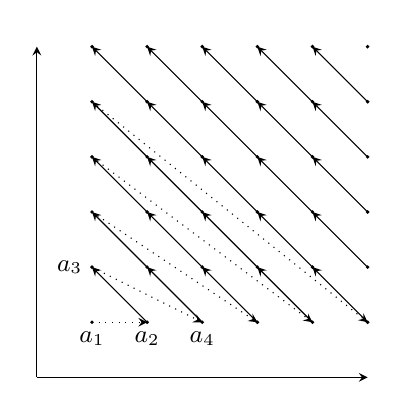
\begin{tikzpicture}[scale=0.7, >=stealth]
    \draw[->] (0, 0) -- (0, 6) node[above] {$\N$};
    \draw[->] (0, 0) -- (6, 0) node[right] {$\N$};

    \node[below] at (1, 1) {\small$a_1$};
    \node[below] at (2, 1) {\small$a_2$};
    \node[left] at (1, 2) {\small$a_3$};
    \node[below] at (3, 1) {\small$a_4$};

    \foreach \x in {1, 2, ..., 6} {
        \foreach \y in {1, 2, ..., 6} {
          \fill (\x, \y) circle (1pt);
          \ifnum \y < 6
            \ifnum \x = 1
              \draw[->, dotted] (\x, \y) -- (\x + \y, 1);
            \else
              \draw[->] (\x, \y) -- (\x - 1, \y + 1);
            \fi
          \fi
        }
    }
  \end{tikzpicture}
  \end{center}
  Define $a_1 = (1, 1)$ and $a_n$ inductively given $a_{n-1} = (p, q)$ by writing:
  \[
    a_n = \begin{cases}
    (p - 1, q + 1) & \text{ if } p \neq 1 \\
    (p + q, 1) & \text{ if } p = 1
    \end{cases}
  \]
  We can show by induction that this list includes every point $(x, y) \in \N \times \N$
\end{proof}
\begin{proof}[Injection]
  \label{ftaInjectiveProof}
  Define $f: \N \times \N \to \N$, $(x, y) \mapsto 2^{x}3^{y}$.
  Then $f$ is injective by the uniqueness of prime factorisations provided by the Fundamental Theorem of Arithmetic (\cref{uniquePrimeFactorisation}).
  So by \cref{countabilityEquivalence}, $\N \times \N$ is countable.
\end{proof}
\begin{corollary}
  $\Z \times \Z$ is countable.
\end{corollary}
\begin{proof}
  Since $\Z$ is countable, there is an injection $f: \Z \to \N$.
  We have just seen that $\N \times \N$ is countable so there is an injection $g: \N \times \N \to \N$.
  Hence, we have an injection:
  \[
    \Z \times \Z \xrightarrow{(f, f)} \N \times \N \xrightarrow{g} \N
  \]
  Thus $\Z \times \Z$ is countable by \cref{countabilityEquivalence}.
\end{proof}
\begin{remark}
  We can iterate this by induction to show that:
  \[
    \Z^{k} = \underbrace{\Z \times \cdots \times \Z}_{k \text{ copies}}
  \]
  is countable for any $k \in \N$.
\end{remark}
\begin{theorem}
  \label{countableUnion}
  A countable union of countable sets is countable.
\end{theorem}
\begin{proof}
  Since there is countably many of them, we may assume that our countable sets are indexed by $\N$.
  So given countable sets $A_1, A_2, \ldots$ (which may terminate) we wish to show that:
  \[
    \bigcup_{n \in \N} A_n \text{ is countable}
  \]
  For each $i \in \N$, since $A_i$ is countable, we may enumerate its elements as $a^{(i)}_{1}, a^{(i)}_{2}, a^{(i)}_{3}, \ldots$ (which may terminate)

  Define $f: \bigcup_{n \in \N} A_n \to \N$, $x \mapsto 2^{i}3^{j}$ where $x = a^{(i)}_{j}$ for the \textbf{least} $i$ such that $x \in A_i$ as $x$ could be in multiple sets, however by WOP, we can pick the least such $i$.
  This is an injection by the same argument as in \cref{ftaInjectiveProof}.

  Alternatively, the association of $x$ with a unique pair $(i, j)$ provides a bijection $\bigcup A_n \to  \N \times \N$, which we know is countable.
\end{proof}
\begin{example}[Countability of $\Q$]
  We can define $\Q$ as:
  \[
    \Q = \bigcup_{n \in \N} \left\{\frac{m}{n}: m \in \Z\right\}
  \]
  This is a countable union of countable sets so $\Q$ is countable.
\end{example}
\begin{theorem}
  The set $\mathbb{A}$ of algebraic numbers is countable.
\end{theorem}
\begin{proof}
  It suffices to show that the set of all polynomials with integer coefficients is countable, as each polynomial has a finite number of roots (by \cref{fact2}), so $\mathbb{A}$ is a countable union of countable sets and is therefore countable by \cref{countableUnion}.

  In fact, it suffices to show that for each $d \in \N$, the set $P_d$ of all integer polynomials of degree $d$ is countable, as then the union of the sets of their roots is a countable union of countable sets.

  The map $P_d \to \Z^{d + 1}$,
  \[
    p(x) = a_d x^{d} + a_{d - 1}x^{d - 1} + \cdots + a_1 x + a_0 \mapsto (a_d, a_{d - 1}, \ldots, a_1, a_0)
  \]
  is an injection as each polynomial is uniquely defined by its coefficients.
  Since $\Z^{d + 1}$ is countable, $P_d$ is countable.
\end{proof}
\section{Uncountable Sets}
\begin{definition}[Uncountable]
  A set is \textit{uncountable} if it is not countable.
\end{definition}
\begin{theorem}
  $\R$ is uncountable.
\end{theorem}
\begin{proof}
  Covered next lecture.
\end{proof}
\end{document}
